\documentclass[]{standalone}

\usepackage{tikz}
\usetikzlibrary{calc}

\begin{document}

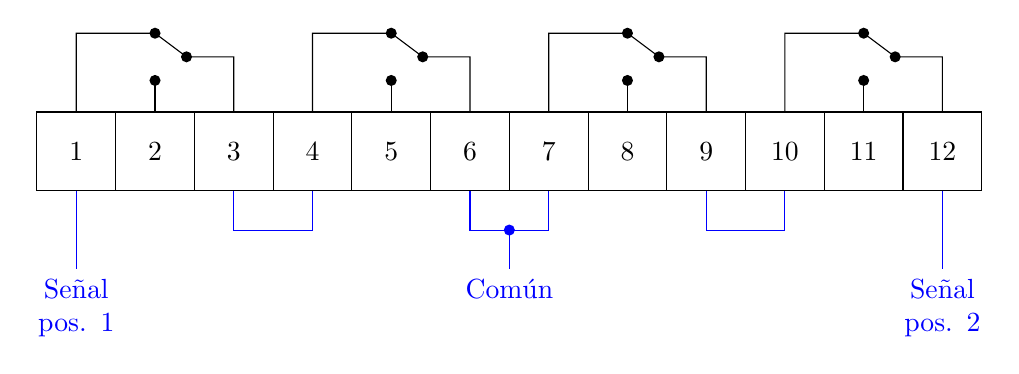
\begin{tikzpicture}
\foreach \x in {1,...,12}
{
	\draw (\x,0) +(-0.5,-0.5) rectangle ++(0.5,0.5);
	\draw (\x,0) node {\x};
}
\foreach \x in {1,4,7,10}
{
	\draw (\x,0.5) |- ++(1,1) -- ++(0.4,-0.3) -| ($(\x,0.5)+(2,0)$);
	\draw (\x,0.5)++(1,0) -- ++(0,0.4);
	\fill (\x,1.5)++(1,0) circle[radius=2pt]
		  (\x,0.9)++(1,0) circle[radius=2pt]
		  (\x.4,1.2)++(1,0) circle[radius=2pt];
}
%\foreach \x in {1,4,7,10}
%{
%	\path
%	(\x,-1) node {NC}
%	++(1,0) node {NA}
%	++(1,0) node {C};
%}
%\draw (1,-1.5) -- ++(0,-0.3) -- node[below] {posición 1} ++(5,0) -- ++(0,0.3);
%\draw (7,-1.5) -- ++(0,-0.3) -- node[below] {posición 2} ++(5,0) -- ++(0,0.3);

%% Cableado %%
\draw[color=blue]
	(1,-0.5) -- ++(0,-1) node[below, text width=1cm, align=center] {Señal pos. 1}
	(12,-0.5) -- ++(0,-1) node[below, text width=1cm, align=center] {Señal pos. 2}
	(3,-0.5) -- ++(0,-0.5) -| (4,-0.5)
	(6,-0.5) -- ++(0,-0.5) -| (7,-0.5)
	(9,-0.5) -- ++(0,-0.5) -| (10,-0.5)
	(6.5,-1) -- ++(0,-0.5) node[below] {Común};
\fill[color=blue]
	(6.5,-1) circle[radius=2pt];
\end{tikzpicture}

\end{document}